\documentclass{beamer}
\usepackage{main}

%%%%%%%%%%%%%%%%%%%%%%%%%%%%%%%%%%%%%%%%%%%%%%%%%%%%%%%%%%%%%%%%%%%%%%%%%%%
% Metadata
%%%%%%%%%%%%%%%%%%%%%%%%%%%%%%%%%%%%%%%%%%%%%%%%%%%%%%%%%%%%%%%%%%%%%%%%%%%

\usetheme{Goettingen}
\title{\textbf{Review}\\Establishment of a Central Process Governance Organization Combined with Operational Process Improvements}
\author{Auer Thomas}
\date{\today}
\institute{University of Klagenfurt}

%%%%%%%%%%%%%%%%%%%%%%%%%%%%%%%%%%%%%%%%%%%%%%%%%%%%%%%%%%%%%%%%%%%%%%%%%%%
% Document start
%%%%%%%%%%%%%%%%%%%%%%%%%%%%%%%%%%%%%%%%%%%%%%%%%%%%%%%%%%%%%%%%%%%%%%%%%%%
\begin{document}

\frame{\titlepage}

\begin{frame}
    \tableofcontents
\end{frame}



\section{Definitions}
\begin{frame}{Definitions}
    \begin{enumerate}[$\circ$]
        \item Operational Process\\An operational process is a method to get a specific, singular task done, such as the assembly of a product. 
        \item Business Process\\A business process is a series of operational processes that result in a specific goal, such as creating and delivering a product or service to a customer.
    \end{enumerate}    
\end{frame}

\begin{frame}{Definitions}
    \begin{enumerate}[$\circ$]
        \item Business Process Management (BPM)\\BPM is concerned with improving a business process from start to finish. (Plan-Do-Act-Check; Design-Model-Execute-Monitor-Optimize; ...)
        \item Business Process Governance (BPG)\\BPG is the practice of overseeing, monitoring, regulating, and managing how business processes are aligned and executed.
    \end{enumerate}    
\end{frame}


\section{Project Introduction}
\begin{frame}{Project Introduction}
    The telecommunication company "ME Telco" adapted to changing market conditions and innovations, to increase competitive advantages, and improve customer satisfaction and operational efficiency.

    \vspace{1em}

    ME Telco is a leading telecommunications operator with more than 100 million customers.
\end{frame}

\begin{frame}{Project Introduction -- Main problems}
    The company suffered from the following issues:
    \begin{enumerate}[$\circ$]
        \item Customer satisfaction on the decline
        \item Competition by innovative market rivals
        \item Requests and incident resolutions took too long
        \item Unclear responsibilities leading to task reassignment
    \end{enumerate}
\end{frame}

\begin{frame}{Project Introduction -- Organizational issues}
    Among the main difficulties for the organization to handle, to alleviate the core issues, are as follows:
    \begin{enumerate}[$\circ$]
        \item Organization's functional structure is oriented around technical infrastructure
        \item Growing complexity was no longer manageable with existing structures
    \end{enumerate}
\end{frame}

\begin{frame}
    \begin{center}
        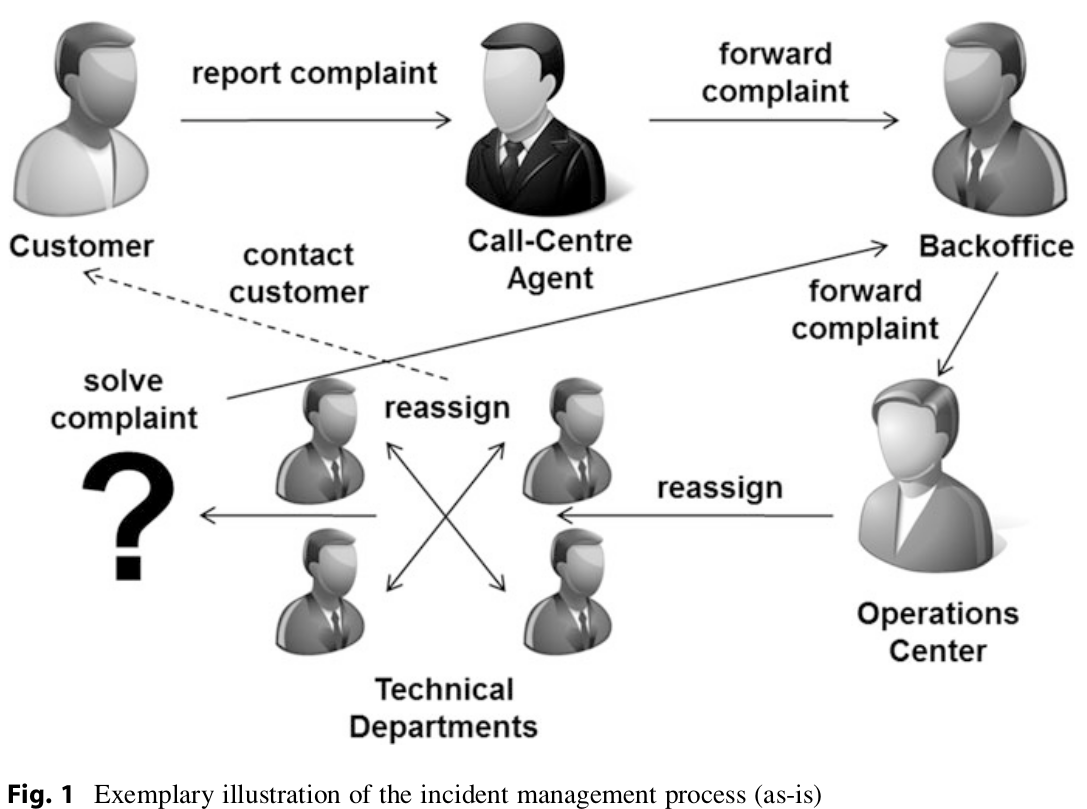
\includegraphics[width=1.0\textwidth]{proj_incidentmgmt.png}
    \end{center}
\end{frame}

\begin{frame}{Project Introduction -- Problem analytics}
    Identification of core problems via BPM diagnostics:
    \begin{enumerate}[$\circ$]
        \item Missing main process management structure\\Each department had it's own silo-oriented process management
        \item Lacking process definition level\\Processes were defined only on operational level
        \item Intransparency\\Activities between departments were not aligned
        \item Responsibility\\Searching for a responsible person was a major effort
        \item Task reassignment\\Many tasks being reassigned, leading to long delays
    \end{enumerate}    
\end{frame}

\section{Problem approach}
\begin{frame}{Problem approach}
    Split the project restructuring into three phases:
    \begin{enumerate}
        \item High-level diagnostics study of present situation utilizing BPM.
        \item Use findings from phase 1 to design, implement and improve BPM.
        \item Monitor results and transition to the line organization
    \end{enumerate}
\end{frame}

\begin{frame}
    \begin{center}
        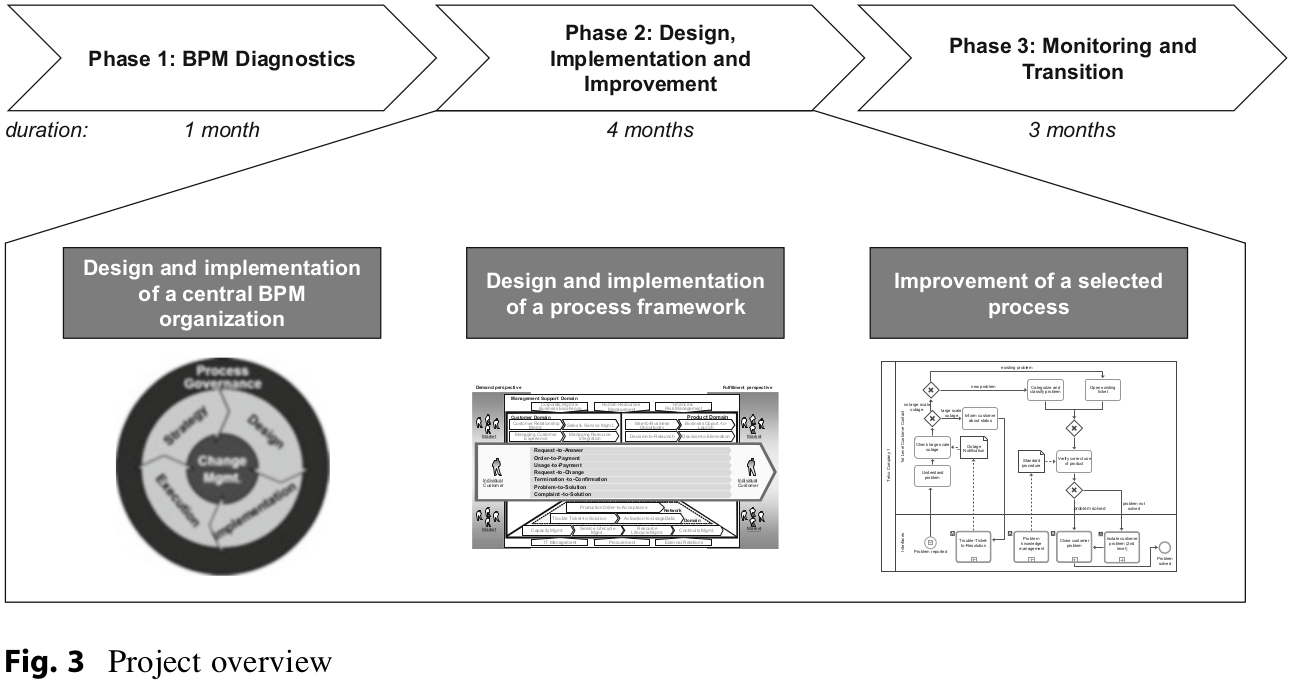
\includegraphics[width=1.0\textwidth]{proj_restructuring.png}
    \end{center}
\end{frame}

\subsection{Phase 1}
\begin{frame}{Problem approach -- 1. Phase}
    BPM diagnostics served as a preliminary assessment based on general maturity criteria.
    It covered organizational responsibilities, methods and tools of BPM, existing process framework, and process reengineering.

    \vspace{1em}

    In summary, findings were related to process ownership, alignment with strategic targets, planning, and future realization of improvement measures.
\end{frame}


\subsection{Phase 2}
\begin{frame}{Problem approach -- 2. Phase}
    Based on Phase 1, Phase 2 consists of 3 objectives:
    \begin{enumerate}[I.]
        \item Development of a central BPM department\\
        \item Development of company-wide process framework\\
        \item Refining of selected processes\\
    \end{enumerate}
\end{frame}

\begin{frame}{I. Development of a central BPM department}
    Create an organizational entity that is responsible for the management and methodical governance of business processes.

    \vspace{1em}

    This encompasses the creation of a BPM department, selecting tools, defining roles and responsibilities, and the development of policies and templates.
\end{frame}

\begin{frame}{II. Development of company-wide process framework}
    Based on the industry-specific process model standard, ''eTOM'', a customized process framework is generated.
    It followed a hierarchical process structure, detailed to level 2 process descriptions for the whole company.

    \vspace{1em}

    This covered identifying and involving appropriate stakeholders, changing employee communication and documents, employee training, and a final approval by the executive board.

\end{frame}

\begin{frame}{III. Refining of selected processes}
    The incident management process was selected as a proof of concept.

    \vspace{1em}

    The process was re-developed through employee training and changes to existing applications.
\end{frame}

\subsubsection{Process Governance}
\begin{frame}{BPM Department \& Governance}
    The new process governance involved the following positions:
    \begin{enumerate}
        \item Process ambassadors\\Responsible for communication and escalations
        \item Process owners\\Senior managers, who had functional responsibility for whole business processes.
        \item Process team leader \& Sub-Process partners\\Design and implementation on operational process level
        \item Business process office\\Responsible for the overall governance
    \end{enumerate}
\end{frame}

\begin{frame}
    \begin{center}
        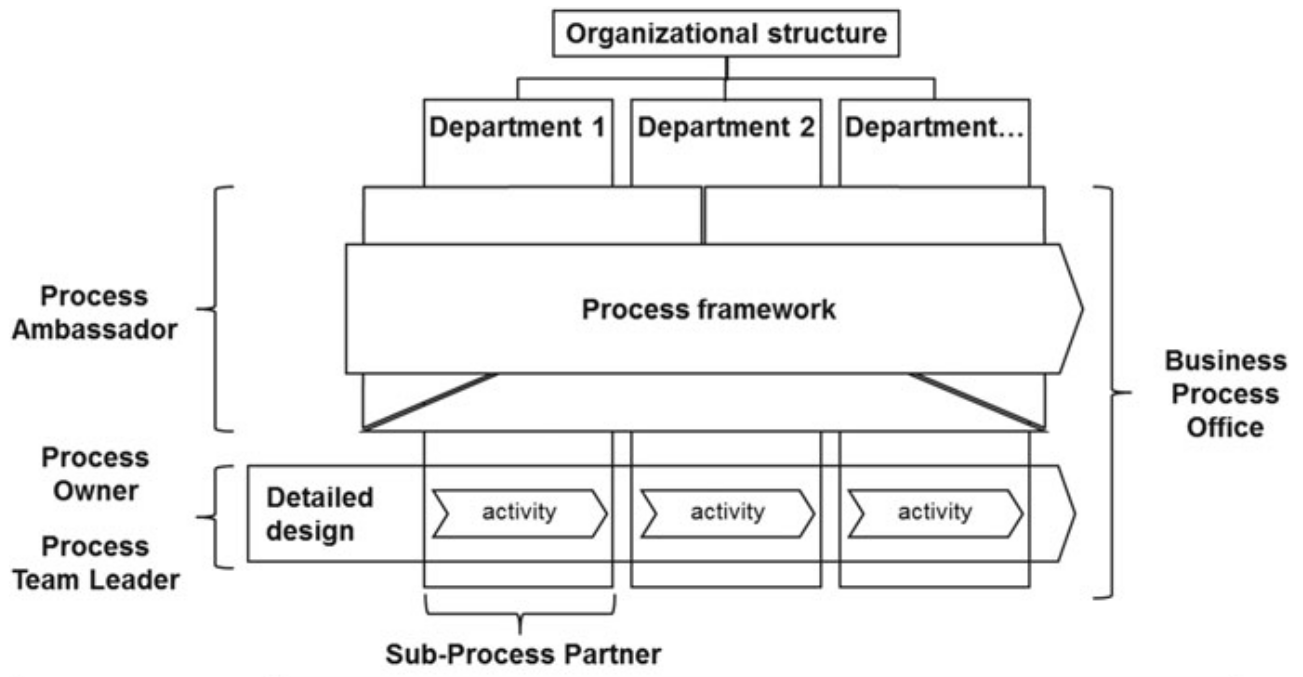
\includegraphics[width=1.0\textwidth]{proj_bpmDepartment.png}
    \end{center}
\end{frame}


\subsubsection{Process Framework}
\begin{frame}{Process Framework}
    A cross-functional process framework was created to bridge the gap between the central BPM department and the operational processes.

    \vspace{1em}

    It provides high-level definitions of all processes based on the eTOM process model.
\end{frame}

\begin{frame}{Process Framework -- Domains}
    The process framework contains five domains:
    \begin{enumerate}[1.]
        \item Customer-centric: Sales and customer service; Tasks started and ended with the customer
        \item Technology: The development and realization of telecommunication services
        \item Product: Design and launch of services, provided by the technology domain
        \item Customer: Market research and campaigns; Supports customer-related activities
        \item Support: General support activities, including finance and human resources
    \end{enumerate}
\end{frame}

\begin{frame}
    \begin{center}
        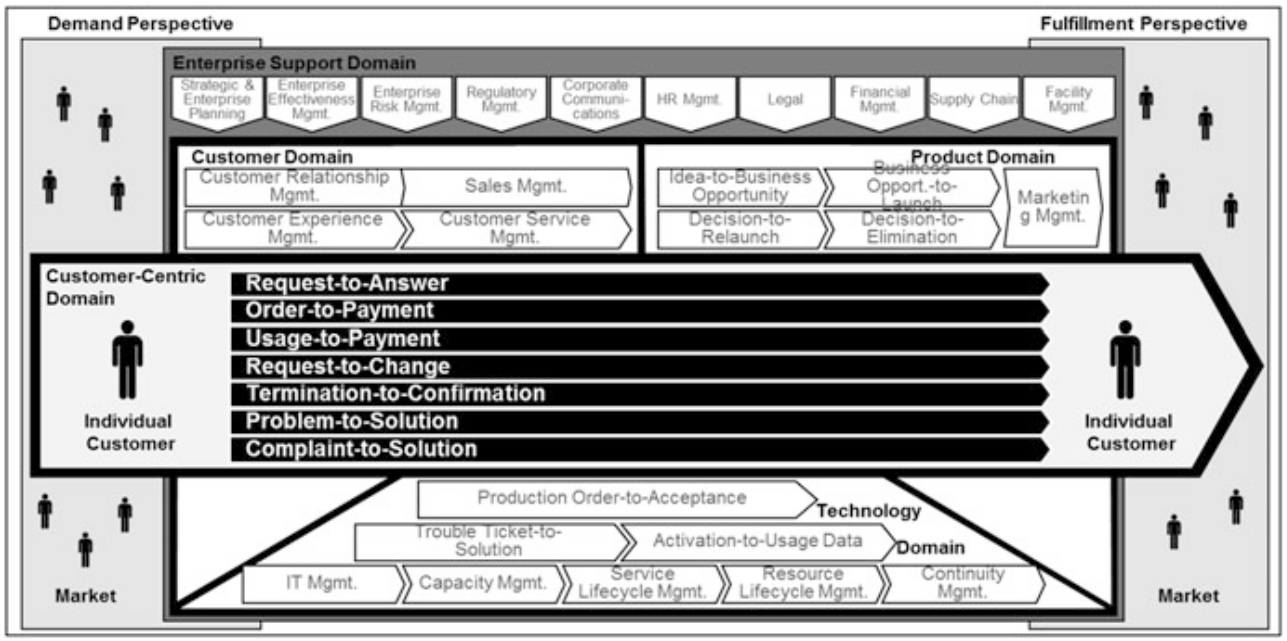
\includegraphics[width=1.0\textwidth]{proj_procFramework.png}
    \end{center}
\end{frame}


\subsection{Phase 3}
\begin{frame}{Phase 3 -- Results monitoring}
    In respect to Phase 2, the following results were achieved:
    \begin{enumerate}
        \item Creation of BPM department
        \item Company-wide process framework was established
        \item Major improvement of the incident management process
    \end{enumerate}
\end{frame}

\begin{frame}
    \begin{center}
        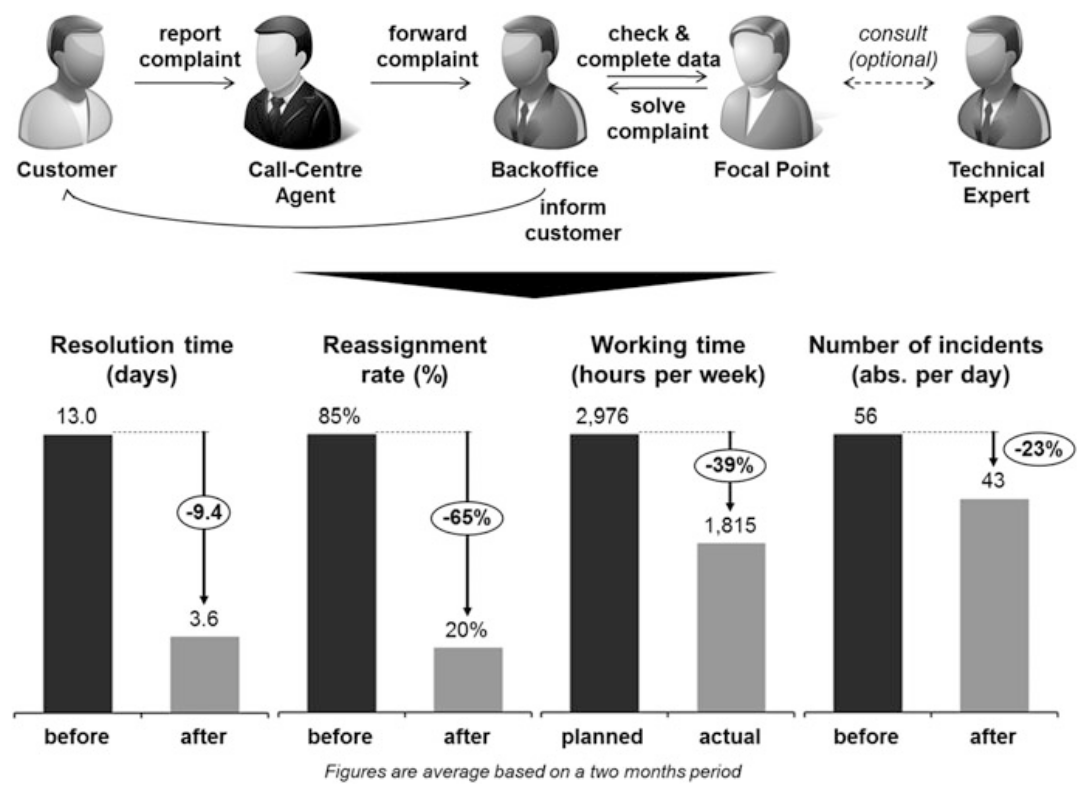
\includegraphics[width=1.0\textwidth]{proj_phase3results.png}
    \end{center}
\end{frame}

\section{Project results}
\begin{frame}{Project results -- Extent of restructuring}
    \begin{enumerate}[$\circ$]
        \item Project duration of 8 months
        \item 18 stakeholder groups were involved
        \item 170 employees received training
        \item 30 interviews and site visits were conducted for as-is analysis
        \item 120 employees received operational training on the new incident management process alone
        \item 8 employees received detailed off-site BPM training
    \end{enumerate}
\end{frame}

\begin{frame}{Project results -- Figures}
    All figures are averages that were calculated based on performance for 2 months before and 2 months after implementation.
    \begin{enumerate}[$\circ$]
        \item Incident resolution time: 13 days $\rightarrow$ 3,6 days
        \item Task reassignment rate: 85\% $\rightarrow$ 20\%
        \item Working hours: 2976 $\rightarrow$  1815
    \end{enumerate}
    Additionally, the numbers of incidents declined by 23\%, presumably due to elimination of repeated reports.
    A positive effect on customer satisfaction was not analyzed, but can be assumed.
\end{frame}

\begin{frame}{Project results -- Additional remarks}
    \begin{enumerate}[$\circ$]
        \item Implementation tasks were partially finished -- 45\% were realized, further 38\% have been started.
        \item Planned changes for application systems were partially -- 40\% were implemented, 60\% required additional budget and/or decisions.
        \item Continous change of organizational positions -- Parallel reorganization initiatives, re-nominations and additional training has to be considered
        \item Future plans were not completely ensured -- Other initiatives were launched during the project that could influence the process management
    \end{enumerate}
\end{frame}

\section{Conclusion}
\begin{frame}{Conclusion}
    From a BPM perspective, the following points can be derived from this study:
    \begin{enumerate}[$\circ$]
        \item Process content is an important factor in BPM implementations
        \item Process ownership requires considerations of different BPM elements
        \item Early involvement of stakeholders is essential
        \item Customization of industry-standard models require transparent decisions and approaches
        \item General BPM governance and methods are important for an operational process improvement
    \end{enumerate}
\end{frame}




\section{Summary}
\begin{frame}{Summary}
A telecommunication company strategically transformed their workflows via business process management (BPM).
    \begin{enumerate}[$\circ$]
        \item \textbf{Problems}\\-- Silo-oriented process management\\-- Missing cross-functional transparency\\-- Lack of assigned responsibility
        \item \textbf{Approach}\\-- Identification of counter-measures\\-- Creation of new organizational unit responsible for central BPM\\-- Monitoring and transfering project results to daily operations
    \end{enumerate}
\end{frame}

\begin{frame}{Summary}
    \begin{enumerate}[$\circ$]
        \item \textbf{Results}\\-- Improve average resolution time from 13 to 3,6 days\\-- Decrease task reassignment rate from 85\% to 20\%\\-- Decrease working time from 2976h to 1815h
        \item \textbf{Outlook}\\-- Process content and management is an significant business success factor\\-- Early involvement of stakeholders is essential\\-- Decision making models require transparency 
    \end{enumerate}
\end{frame}

\begin{frame}
    \centering \textbf{Thank you for your attention}
\end{frame}


\end{document}